\chapter{Metodi di Risoluzione Simbolica}

\section{Motivazioni}

L'analisi simbolica di circuiti elettrici rappresenta una tecnica formale per lo studio di questi ultimi, fornendo un'ampia gamma di informazioni utili sulle diverse caratteristiche del circuito stesso. Tale tecnica ha visto negli anni l'alternarsi di periodi di fervida attenzione a momenti di blanda considerazione, prevalentemente a causa della complessità computazionale che, col passare del tempo, è diventata uno scoglio sormontabile data la crescente potenza di calcolo a disposizione, riportando in auge l'argomento.\\
L'analisi simbolica può essere usata per lo studio di comportamenti specifici o caratteristiche legate alle variabili dipendenti, le variabili indipendenti e a tutti gli altri elementi che concorrono a comporre un circuito. A differenza e in aggiunta a ciò che si propone di fare l'analisi numerica (che oltre ad offrire migliori prestazioni in termini prettamente computazionali, permette di ispezionare il comportamento di un circuito sotto svariati aspetti), l'approccio simbolico aiuta lo sviluppatore a comprendere meglio quali elementi incidano effettivamente, in modo più o meno significativo, su tale comportamento. Da notare che, sebbene ad oggi lo studio simbolico sia limitato ad un ben definito insieme di elementi, è possibile avvicinare anche oggetti altrimenti al di fuori dalla portata dello strumento attraverso approssimazioni note nell'ambito elettronico. A supporto di questa tesi, si possono considerare ad esempio le approssimazioni per piccoli segnali e il modello di Giacoletto (per le alte frequenze) utili all'approssimazione di transistor a giunzione.

\begin{figure}[hb]
 \centering
 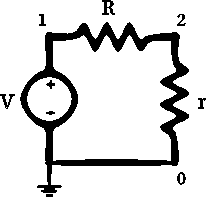
\includegraphics{immagini/vdiv.pdf}
 \caption{Partitore di tensione}
 \label{fig:vdiv}
\end{figure}

Nonostante la complessità degli algoritmi sviluppati negli anni, tale metodologia offre la possibilità di un'analisi veramente flessibile ed esclusiva, riservata ai soli componenti di interesse. Dall'analisi simbolica si possono infatti ricavare diverse forme di espressione per le variabili d'interesse di un circuito. Si consideri a tal proposito il semplice partitore di tensione in figura \ref{fig:vdiv}, supponendo di voler attribuire una rappresentazione simbolica al generatore di tensione $V$ e alla resistenza $R$, trattando invece la resistenza $r$ come valore numerico, poiché in essa non è riposto alcun interesse. Poniamo inoltre che il generatore abbia come valore numerico 3 V, la prima resistenza 5 \ohm\ e la seconda resistenza 1 \ohm.\\
Otteniamo attraverso la risoluzione simbolica, banalmente, tre forme anziché una per la funzione di trasferimento.\\
Più nello specifico avremo una forma puramente simbolica, ovvero: $$ \frac{V * r}{R + r} $$
Una forma ricavata sostituendo ad ogni elemento la sua rappresentazione numerica, come segue: $$ \frac{3 * 1}{1 + 5} = \frac{1}{2} $$
Infine una forma mista che, una volta compressa e semplificata (minimizzandola e rendendola più comprensibile all'essere umano), meglio rappresenta e si plasma sulla base delle intenzioni dell'utente: $$ \frac{V * 1}{R + 1} = \frac{V}{R + 1} $$

La forma mista sintetizza, di fatto, il comportamento del circuito mettendo in evidenza le sole variabili di interesse e trattando come numeriche, attraverso opportune sostituzioni, tutte le altre. Risulta importante sottolineare l'accenno fatto sopra alle operazioni di compressione e semplificazione. Uno dei rischi in cui si incorre è, infatti, quello di ricavare da tali procedure formule di dimensioni notevoli e difficili da interpretare. Tali formule, attraverso opportune riduzioni, risulterebbero di gran lunga più facilmente gestibili. Pertanto i passi di semplificazione delle espressioni non vanno trascurati poiché anch'essi molto importanti nella catena di sviluppo del risultato.

\paragraph{}
Un altro aspetto da non tralasciare, che non traspare da quanto introdotto finora, è dato dalla possibilità di portare avanti operazioni di analisi numerica sulle formule ottenute. Può sembrare scontato ma la sola osservazione della forma mista richiesta può dare indicazioni all'utente su chi influenza il comportamento del circuito senza esplicarne il come. Del resto anche questa è una informazione interessante e l'analisi simbolica ci viene incontro fornendo la possibilità di ottenere curve di ogni genere al variare dei parametri, così da ricercare quella che meglio approssima il comportamento desiderato. Gestendo infatti formule miste si può procedere banalmente alla sostituzione progressiva di valori associati ai componenti, con l'analisi in determinati intervalli di frequenze e così via.\\
Nulla vieta, in effetti, di effettuare con una forma mista o simbolica tutte o gran parte di quelle operazioni che si possono svolgere di norma con un risolutore numerico.

\paragraph{}
Riassumendo, quindi, è possibile trovare nell'uso di risolutori simbolici (anziché numerici) una maggiore flessibilità per quanto riguarda l'approccio e lo studio del problema, avendo la possibilità di sondarlo da diversi punti di osservazione. Di contro, però, non va trascurata la maggiore richiesta computazionale per questo tipo di analisi che, pertanto, va usata laddove vi sia veramente bisogno.\\
Un approccio plausibile potrebbe essere quello di un'analisi a più fasi durante le quali, in base alle necessità e ai problemi che si propongono, si affronta lo studio attraverso risolutori prettamente simbolici o prettamente numerici. Sconsigliato l'uso di un risolutore simbolico in ambiti dove vi sia la necessità della sola analisi numerica e, viceversa, l'uso di risolutori numerici non è possibile se si hanno richieste di analisi simbolica.

\paragraph{}
Molto importante è capire che i due strumenti, risolutori simbolici e numerici, non sono alternativi ma complementari ed entrambi arricchiscono il parco di oggetti che un progettista può avere a disposizione per assolvere al suo compito.


\section{Cenni storici}

Le metodologie di analisi numerica si sono evolute negli anni, migrando addirittura da un ambito prevalentemente matematico (dove si procedeva con operazioni matriciali) allo spazio dei grafi. In quest'ultimo ambito, in particolare grazie ai contributi ottenuti prima da Grimbleby \cite{Grimbleby} e quindi da Schach \cite{MRT}, sono state notevolmente abbattute le barriere di complessità computazionale, aspetto che, in concomitanza alla sempre crescente potenza di calcolo a disposizione, ha permesso lo sviluppo di nuovi e performanti algoritmi, tutt'oggi in uso.

L'analisi simbolica dei circuiti elettrici tiene banco nell'ambiente elettronico fin dagli anni '70, poiché risultano innegabili i vantaggi che essa può portare se affiancata all'analisi numerica. Del resto, come già anticipato, fin dagli albori ha trovato estimatori nell'ambito teorico e critici nell'ambito pratico, risultando praticamente inattuabile se non a circuiti dalle dimensioni estremamente limitate e per i quali, di fatto, non risultasse realmente necessaria.

Le metodologie di risoluzione proposte hanno trovato terreno fertile prevalentemente in due aree tematiche, rendendosi note attraverso i \textit{metodi algebrici} e i \textit{metodi topologici}.

Senza addentrarsi nello specifico, la prima categoria ricavava le formule desiderate attraverso tecniche di manipolazione simbolica delle espressioni algebriche applicate alle equazioni della rete. Ciò richiedeva al contempo un grosso impegno computazionale e grandi quantitativi di memoria, tanto per la memorizzazione quanto per l'elaborazione. I metodi algebrici hanno quindi ceduto il passo ai metodi topologici. Questi ultimi hanno permesso di snellire i processi di risoluzione (guadagnando in termini di risorse di calcolo), per la memorizzazione e per l'espletamento delle proprie funzioni. Uno dei primi esempi applicabili in tal senso è citato in \cite{Grimbleby} e sviluppato in \textit{Sapec}\graffito{Sapec (Symbolic Analysis Program for Electric Circuits) è un risolutore simbolico privo di interfaccia grafica, che riceve dati in ingresso come parametri da riga di comando}, cuore del software \textit{SapWin}\graffito{SapWin (Symbolic Analysis Program for Windows) è un'interfaccia sviluppata per ed intorno a Sapec ed invoca quest'ultimo nelle fasi di risoluzione} ed entrambi predecessori di \textit{QSapecNG}, il quale implementa invece al suo interno un'evoluzione dell'algoritmo di cui sopra, come proposta in \cite{MRT}. Scendendo un po' più nel dettaglio dei metodi topologici, bisogna osservare che un attento studio delle strutture dati, delle relazioni fra esse e dei metodi di accesso alle informazioni può portare a notevoli migliorie sotto ogni aspetto. Anche per questo tali metodologie hanno trovato largo consenso e suscitato l'interesse di studiosi tuttora intenti a perfezionarne il comportamento. Basti pensare infatti che, sotto determinate condizioni, i metodi topologici si riducono ad algoritmi su grafi pesati (che rappresentino opportunamente il circuito in esame). A tali grafi e algoritmi possono pertanto essere applicate tutte le tecniche di compressione e ottimizzazione conosciute, guadagnando ulteriormente in prestazioni.

\paragraph{}
Da quanto brevemente detto si intuisce come sia vivo e vitale il mondo intorno a questa categoria di problemi, anche a causa dell'importanza non relegata esclusivamente all'ambito accademico ma estesa anche a quello commerciale. Purtroppo, però, la complessità del problema affrontato è tale da rendere difficoltoso il cammino e difficile il processo evolutivo degli algoritmi coinvolti.


\section{Da Sapec a QSapecNG, attraverso SapWin}

Per quanto riguarda la storia legata al software qui discusso, esso nasce, cresce e si sviluppa interamente all'interno dell'Università degli Studi di Firenze. \textit{SapWin} si appoggia sul motore di analisi \textit{Sapec}, un software separato dall'interfaccia grafica per scelta degli sviluppatori e attraverso l'uso di quest'ultimo arriva fino all'attuale versione 3.0, ampliando il suo parco di funzionalità ma senza sostituire l'algoritmo che fa da base al processo di risoluzione. Eppure tanto SapWin quanto Sapec rappresentano il frutto di anni di studi teorici e implementazioni pratiche dei loro padri.\\
Una discussione sul mondo di SapWin esula però da questo lavoro e richiederebbe svariati capitoli per poter sciogliere tutti i nodi.

Nel suo piccolo, invece, \textit{QSapecNG} nasce come il frutto di un lavoro iniziato durante il percorso di studi triennale dell'autore, conclusosi in una prima fase con lo sviluppo di SapecNG. Quest'ultimo era costituito da un motore di risoluzione scritto in C e un semplice parser LALR (\textit{LookAhead Left to Right parser}) basato su \textit{flex/bison}\graffito{Flex (Fast Lexical Analyzer) e Bison (GNU Parser Generator) sono una coppia consolidata nel mondo dei compiler-compiler o generatori di compilatori}, era in grado di elaborare i file prodotti in forma di \textit{netlist} da SapWin e quindi catturare le informazioni richieste restituendole all'utente. La peculiarità di SapecNG non risiedeva però tanto in funzionalità particolari messe a disposizione, strumenti innovativi utilizzati od ottimizzazioni di alcun genere, bensì nello sviluppo di un algoritmo che migliorasse le prestazioni di Sapec: da questo la decisione della dicitura \textit{NG}, o \textit{Next Generation}, a simboleggiare il passo avanti in termini di evoluzione fatto nell'ambito del progetto in seno all'Università di Firenze. Altra caratteristica importante e mantenuta nel tempo era la sua portabilità, ad oggi e sempre più un aspetto necessario per programmi di nuova generazione. La carenza principale di SapecNG risiedeva nella possibilità di utilizzo da sola riga di comando e nella troppa rigidità del codice, il che rendeva il software utile al solo scopo didattico.

Con QSapecNG vi è stata una riscrittura per intero del software SapecNG, migrando il codice da C a C++ e sfruttando le potenzialità offerte da librerie esterne quali \textit{Boost C++} \cite{BGL} e il framework \textit{Qt} \cite{Qt}. L'attenzione al design ha mantenuto una netta separazione fra backend e frontend, così da permettere in futuro la riscrittura di una GUI anche attraverso diverse librerie e al contempo dando la possibilità di evolvere il motore sottostante e le funzionalità offerte senza incidere in maniera significativa o difficilmente gestibile sull'interfaccia utente. Le tecniche di sviluppo del software e i pattern più o meno noti applicati, hanno permesso di rendere elegantemente complicati alcuni frangenti altrimenti ostici. Infine, anche in QSapecNG è stata mantenuta la portabilità del codice.\\
In definitiva QSapecNG si propone oggi come una soluzione multipiattaforma per la risoluzione simbolica di circuiti elettrici e, pur essendo un cantiere aperto a nuove possibilità di espansione, offre già un'ampia gamma di strumenti e ingloba tecniche di sviluppo mirate a semplificare la sua crescita e l'aggiunta di componenti.


\section{Scopo del lavoro di tesi}

Il lavoro di tesi si colloca a metà fra la teoria e la pratica, arricchendo, approfondendo e rendendo fruibile quanto proposto in letteratura. L'obiettivo è stato principalmente quello di far incontrare strumenti di analisi simbolica e sistemi emergenti (quali i sistemi \textit{Unix-like}), offrendo allo stesso tempo l'opportunità di usare algoritmi e ambienti all'avanguardia. Questa strada è stata percorsa per lunghi tratti, arrivando a sviluppare un software innovativo, flessibile ed in grado di proporsi come un ambiente di test e sviluppo dove possano sfociare in futuro applicazioni pratiche derivate da studi teorici.

Nei prossimi capitoli e nelle appendici sarà discusso quanto segue:
\begin{description}
 \item[Studi teorici] Illustrazione delle tecniche di sintesi dei componenti (e quindi di un circuito) in forma di coppia di grafi in corrente e in tensione, algoritmi per la ricerca degli alberi di copertura comuni fra due grafi e studio delle metodologie per il calcolo corretto delle formule di trasferimento.
 \item[Esempi] Verrà illustrato un piccolo esempio modello che, seguendo le linee teoriche, presenti praticamente il procedimento utilizzato per l'analisi simbolica di un circuito.
 \item[Frameworks] Saranno introdotti i principali \textit{frameworks} di sviluppo utilizzati per passare effettivamente dalla teoria alla pratica.
 \item[Tecniche di programmazione] Verranno dati alcuni cenni sulle principali tecniche di programmazione adottate e sulle soluzioni più eleganti e flessibili presenti nel codice.
 \item[Generazione automatica degli schemi] Uno studio proposto nell'ambito della ricerca operativa, allo scopo di ricostruire uno schema per circuiti elettrici (definiti tramite file di testo) che abbatta l'occupazione di spazio dislocando in modo ottimo i diversi componenti.
\end{description}
